

%*******************************************************
% This program is free software: you can redistribute it and/or modify
% it under the terms of the GNU General Public License as published by
% the Free Software Foundation, either version 3 of the License, or
% (at your option) any later version.
%
% This program is distributed in the hope that it will be useful,
% but WITHOUT ANY WARRANTY; without even the implied warranty of
% MERCHANTABILITY or FITNESS FOR A PARTICULAR PURPOSE.  See the
% GNU General Public License for more details.
%
% You should have received a copy of the GNU General Public License
% along with this program.  If not, see <http://www.gnu.org/licenses/>.
%************************************************
\chapter{This is chapter four}
\label{ch:name4}
%************************************************

\begin{flushright}
{\slshape Lorem ipsum dolor sit amet, consectetuer adipiscing.}\\
{\slshape Aenean commodo ligula eget dolor. Aenean massa.}\\
% This generate dummy text. Remove this line and replace by your quote.
\medskip
--- John Doe,\\
Unified Theory of the Important Theories,\\
{\slshape An Important Journal},\\
Vol.~123, pp.~1234--1243, Dec.~2016.\\
\end{flushright}

\bigskip


%\minitoc\nomtcpagenumbers

%\marginpar{\myTitle \myVersion}

\section{Introduction}
\label{sec:ch_4_introduction}

\citet{Berg2016} argues that this is a topic sentence followed by explanation, elaboration and examples to introduce the next three subsections. The last sentence of this paragraph shall introduce the next paragraph. \lipsum[1]

This is a topic sentence followed by explanation, elaboration and examples to introduce the next three subsections \citep{Collins2016}. The last sentence of this paragraph shall introduce the next paragraph. \lipsum[1]

\citet{Graham2016} and \citet{Grant2016} assert that this is a topic sentence followed by explanation, elaboration and examples to introduce the next three subsections. The last sentence of this paragraph shall introduce the next paragraph. \lipsum[1]

\section{First main stuff}
\label{sec:ch_4_firstmain}

This is a topic sentence followed by explanation, elaboration and examples to introduce this paragraph \citep{Haney2016}. The last sentence of this paragraph shall introduce the next paragraph. \lipsum[1]

This is a topic sentence followed by explanation, elaboration and examples to introduce this paragraph \citep{Jordan2016,Morgan2016}. The last sentence of this paragraph shall introduce the next paragraph. \lipsum[1]

This is a topic sentence followed by explanation, elaboration and examples to introduce this paragraph. The last sentence of this paragraph shall introduce the next paragraph. \lipsum[1]

\section{Second main stuff}
\label{sec:ch_4_secondmain}

This is a topic sentence followed by explanation, elaboration and examples to introduce this paragraph \citep{Scott2016}. The last sentence of this paragraph shall introduce the next paragraph. \lipsum[1]

\begin{figure}[h]
    \centering
    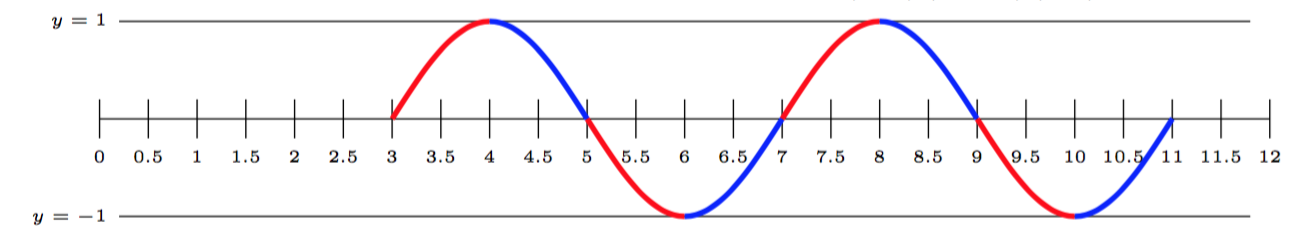
\includegraphics[width=0.9\textwidth]{imageFiles/imageExample}
    \caption{A copy from previous image}
    \label{fig:copycurve}
\end{figure}
 
As \citet{Wells2016} and \citet{Williamson2016} denotated in the figure \ref{fig:copycurve}, the 
function grows near 0. Also, in the page \pageref{fig:curve} 
is the same example in figure \ref{fig:curve}.

This is a topic sentence followed by explanation, elaboration and examples to introduce this paragraph \citep{Stewart2016}. The last sentence of this paragraph shall introduce the next paragraph. \lipsum[1]

This is a topic sentence followed by explanation, elaboration and examples to introduce this paragraph \citep{Gallagher2016}. The last sentence of this paragraph shall introduce the next paragraph. \lipsum[1]

\section{Third main stuff}
\label{sec:ch_4_thirdmain}


This is a topic sentence followed by explanation, elaboration and examples to introduce this paragraph. The last sentence of this paragraph shall introduce the next paragraph. \lipsum[1]

This is a topic sentence followed by explanation, elaboration and examples to introduce this paragraph. The last sentence of this paragraph shall introduce the next paragraph. \lipsum[1]

This is a topic sentence followed by explanation, elaboration and examples to introduce this paragraph. The last sentence of this paragraph shall introduce the next paragraph. \lipsum[1]

\section{Summary}
\label{sec:ch_4_summary}


This is a topic sentence followed by explanation, elaboration and examples to summarise the second subsection. The last sentence of this paragraph shall introduce the next paragraph. \lipsum[1]

This is a topic sentence followed by explanation, elaboration and examples to summarise the third subsection. The last sentence of this paragraph shall introduce the next paragraph. \lipsum[1]

This is a topic sentence followed by explanation, elaboration and examples to summarise the fourth subsection. The last sentence of this paragraph shall introduce the next chapter. \lipsum[1]



%*****************************************
%*****************************************
%*****************************************
%*****************************************
%*****************************************




